%%% Ne pas modifier jusqu'à la ligne 25
\documentclass[a4paper,12pt]{book}
\usepackage[utf8]{inputenc}
\usepackage[french]{babel}
%%\usepackage{CJK}
\usepackage{yhmath}
\usepackage[left=2cm,right=2cm,top=3cm,bottom=2cm, headheight=1.5cm,headsep=1.5cm]{geometry}
%%\usepackage{CJKutf8}
\usepackage{amsfonts}
\usepackage{mathrsfs}
\usepackage{amsmath,amsfonts,amssymb,dsfont}
\usepackage{graphicx}
\usepackage{subfigure}
\usepackage{enumitem}		%\enumerate-resume
\usepackage[colorlinks=true,unicode={true},hyperindex=false, linkcolor=blue, urlcolor=blue]{hyperref}
\newcommand{\myref}[1]{\ref{#1} page \pageref{#1}}

\addto\captionsfrench{\def\tablename{Tableau}}  %légendes des tableaux
\renewcommand\thesection{\Roman{section}~-~} 
\renewcommand\thesubsection{\Roman{section}.\Alph{subsection}~-~} 
\renewcommand\thesubsubsection{\Roman{section}.\Alph{subsection}.\arabic{subsubsection}~-~} 

\newcommand{\conclusion}[1]{\newline \centerline{\fbox{#1}}}

\setcounter{secnumdepth}{3}
\parindent=0pt

\usepackage{fancyhdr}
\pagestyle{fancy}

\lhead{SJTU-ParisTech} 
%%%%%%%%%%%%%%%%%%%%%%%%%%%%%%%%%%
\chead{DM1}
\rhead{Daniel 518261910024}

\begin{document}
\renewcommand{\labelitemi}{$\blacktriangleright$}
\renewcommand{\labelitemii}{$\bullet$}


\section{Exercice 1-2 : Equilibrage d'une machine tournante}
\begin{figure}[h]
    \begin{center}
    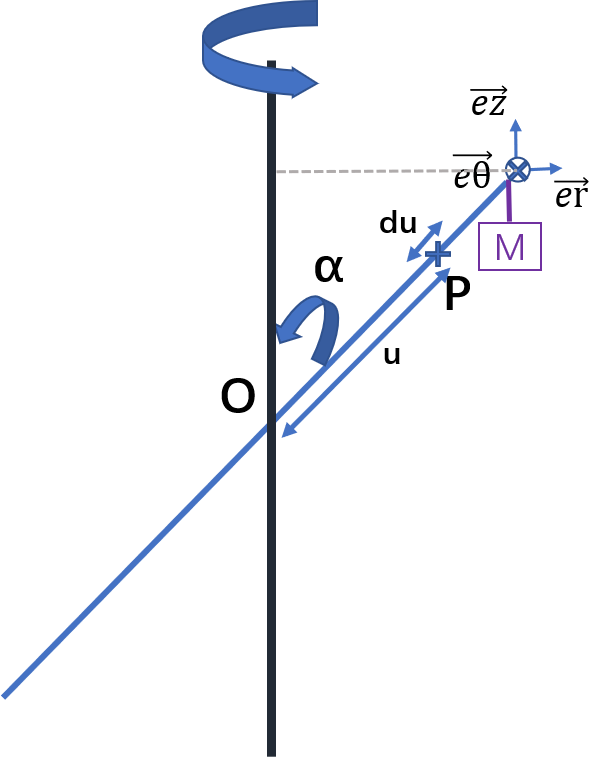
\includegraphics[scale=0.6]{meca2.png}
    \end{center}
    \caption{la barre étudiée}
\end{figure}
\subsection{}
\begin{itemize}
    \item système $(\Sigma)$: la barre de masse $m$ qui tourne autour d'un axe, sa masse lilinéique $\rho=\frac{m}{2L}$
    \item référentiel du laboratoire $(R)$, galiléen, de repère $(O,(\vec{e_u},\vec{e_v},\vec{e_z}))$
\end{itemize}
Dans la base cylindrique, on a 
$$
\frac{d\vec{e_r}}{dt}=\vec{e_\theta}\quad \frac{d\vec{e_\theta}}{dt}=-\vec{e_r}\quad \frac{d\vec{e_z}}{dt}=\vec{0} 
$$


Pour le point matériel $P$ sur la barre, on a sa position
$$
\overrightarrow{OP}=u\sin\alpha \vec{e_r}+u\cos\alpha\vec{e_z}
$$
donc sa vitesse
$$
\overrightarrow{v}_{(R)}(P)=\frac{d\overrightarrow{OP}}{dt}=usin\alpha \omega \vec{e_\theta}
$$
Donc l'énergie cinétique
\begin{align*}
    E_c(\Sigma)&=\int_{(\Sigma)}\frac{1}{2}||\overrightarrow{v}_{(R)}(P)||^2dm_P\\
    &=\int^L_{-L}\frac{1}{2}u^2\sin^2\alpha\omega^2\frac{m}{2L}du\\
    &=\boxed{\frac{u^2\sin^2\alpha\omega^2mL}{6}}
\end{align*}
\subsection{}
Sa moment cinétique
\begin{align*}
\vec{L}_{O,(R)}(\Sigma)&=\int_{(\Sigma)}\overrightarrow{OP}\wedge\vec{v}_{(R)}(P)dm_P\\
&=\int^L_{-L}(u\sin\alpha \vec{e_r}+u\cos\alpha\vec{e_z})\wedge(usin\alpha \omega \vec{e_\theta})dm_P\\
&=\vec{e_z}\int^L_{-L}\omega u^2\sin^2\alpha dm_P-\vec{e_r}\int^L_{-L}\omega u^2\sin\alpha\cos\alpha dm_P\\
&=\boxed{\frac{\omega\sin\alpha mL^2}{3}(\sin\alpha\vec{e_z}-\cos\alpha\vec{e_r})}
\end{align*}
\subsection{}
le moment dynamique
\begin{align*}
\frac{d\vec{L}_{O,(R)}(\Sigma)}{dt}&=\frac{\omega\sin\alpha mL^2}{3}\frac{d}{dt}(\sin\alpha\vec{e_z}-\cos\alpha\vec{e_r})\\
&=\boxed{-\frac{mL^2\omega^2\sin\alpha\cos\alpha}{3}\vec{e_\theta}}
\end{align*}
Le moment dynamique est parallèle à la direction de sa vitesse, qui rotate autour de $O_z$, 
donc 

\fbox{$\vec{L}_{O,(R)}(\Sigma)$ est en précession autour de $O_z$}
% On note $(O,(\vec{\mu_x^{'}},\vec{\mu_y^{'}},\vec{\mu_z^{'}})$ le repère Descartes, avec $\vec{\mu_y^{'}}$ dans le 
% plan $(A)$ qui contient la barre et l'axe. 

% On a donc 
% $$
% \left\{  
%              \begin{array}{l}  
%              \vec{e_u}=\sin{\alpha} \vec{\mu_y^{'}}+\cos \alpha \vec{\mu_z^{'}}\\  
%              \vec{e_v}=\vec{\mu_x^{'}}\\  
%              \vec{e_z}=\cos \alpha \vec{\mu_y^{'}}-\sin \alpha \vec{\mu_z^{'}}  
%              \end{array}  
% \right.  
% $$
% avec 
% $$
% \left\{  
%              \begin{array}{l}  
%                 \vec{\mu_x^{'}}=\cos \theta \vec{\mu_x}+\sin\theta \vec{\mu_y}\\  
%                 \vec{\mu_y^{'}}=-\sin \theta \vec{\mu_x}+\cos\theta \vec{\mu_y}\\   
%                 \vec{\mu_z^{'}}=\vec{\mu_z}
%              \end{array}  
% \right.  
% $$
% Soit le point matériel $P$ tel que $\overrightarrow{OP}=u\vec{e_u}$, donc 
% \begin{align*}
%     \vec{v}_{(R)}(P)&=\frac{d}{dt}\overrightarrow{OP}\\
%     &=u\frac{d}{dt}\vec{e_u}\\
%     &=u\frac{d\theta}{dt}\frac{d}{d\theta}\vec{e_u}\\
%     &=u\omega \sin\alpha\frac{d}{d\theta}\vec{\mu_y^{'}}\\
%     &=-u\omega \sin\alpha\vec{e_v}
% \end{align*}
% On a donc l'énergie cinétique 
% \begin{align*}
%     E_c&=\int_{(\Sigma)}\frac{1}{2}||\vec{v}_{(R)}(P)||^2\,dm_P\\
%     &=\int_{-l}^{l} \frac{1}{2}u^2\omega^2\sin^2\alpha \rho\,du\\
%     &=\boxed{\frac{ml^2\omega^2\sin^2\alpha}{6}}
% \end{align*}
% avec $m=\rho*2l$
% \subsection{}
% On a le moment cinétique
% \begin{align*}
%     \vec{L}_{O,(R)}(\Sigma)&=\int_{(\Sigma)}\overrightarrow{OP}\wedge \vec{v}_{(R)}(P)\,dm_P\\
%     &=\int_{-l}^{l} u\vec{e_u}\wedge(-u\omega\sin\alpha \vec{e_v}) \rho\,du\\
%     &=\boxed{\frac{-ml^2\omega\sin\alpha}{3}\vec{e_z}}
% \end{align*}
% \subsection{}
% On a le moment dynamique 
% \begin{align*}
%     \left(\frac{d\vec{L}_{O,(R)}(\Sigma)}{dt}\right)_{(R)}
%     &=\frac{-ml^2\omega\sin\alpha}{3}\frac{d}{dt}\vec{e_z}\\
%     &=\frac{-ml^2\omega\sin\alpha}{3}\omega \cos\alpha(-\vec{\mu_x^{'}})\\
%     &=\boxed{\frac{ml^2\omega^2\sin\alpha}{3} \cos\alpha\vec{e_v}}
% \end{align*}
% Le moment dynamique est parallèle à la direction de sa vitesse, qui rotate autour de $O_z$, 
% donc 

% \fbox{$\vec{L}_{O,(R)}(\Sigma)$ est en précession autour de $O_z$}
\subsection{}
Pour que la barre reste à l'équilibre, il faut $\vec{F}_{ext \to (\Sigma)=0}$, on a donc la force 
exercé par l'axe sur la barre $\boxed{\vec{F}_{(R),axe \to (\Sigma)}=-\vec{F}_{pes}=mg\vec{e_z}}$

Pour annuler leur moment en $O$, on peut suspendre un objet de masse $M$, qui vérifie $\vec{M}_{O,tot \to (R)}(\Sigma)=0$, donc 
\begin{align*}
\vec{M}_{O,M \to (R)}(\Sigma)&=(L\sin\alpha \vec{e_r}+L\cos\alpha\vec{e_z})\wedge(-Mg\vec{e_z})\\
&=-MgL\sin\alpha(-\vec{e_\theta})
\end{align*}
car le moment de poids est nul, on a donc $Mgl \sin{\alpha}\vec{e_\theta}-\frac{mL^2\omega^2\sin\alpha\cos\alpha}{3} \vec{e_\theta}$, 
d'où $\boxed{M=\frac{mL\omega^2\cos\alpha}{3g}}$
\end{document}